\documentclass[11pt]{scrartcl}
\usepackage{dominatrix}
\usepackage{colortbl}
\usepackage{pgfplots}
\newcommand{\jon}{Jón }
\pgfplotsset{compat=1.9}
\renewcommand\thesubsection{\alph{subsection}}
\definecolor{light-gray}{gray}{0.75}
\title{Production}
\subject{ECON W3213 Spring 2014 \jon Steinsson}
\author{Linan Qiu, lq2137}
\begin{document}
\maketitle

\begin{abstract}
This set of recitation notes covers \textbf{Production}. This is in no way a substitute for attending lectures, but just in case you dozed off or checked your boyfriend's Facebook page while \jon was working Calculus magic on the board, this set of notes should save you.
\end{abstract}

\section{Production Function}

Let's say that you're from Insomnialand, and you survive on cookies and only on cookies. We represent the amount of cookies you produce by the letter $Y$. This is your output.

The amount of cookies you produce depend on the amount of machinery (capital) $K$ you have, and the amount of people you slave drive to produce cookies $L$. 

Hence, we say that 

\[Y = F(K,L) \]

You should always think of output in terms of cookies -- so that you remember that we're always talking about \textbf{real output}. Remember \jon always says, "Let's set relative prices to 1." Effectively, he's saying that you price everything relative to that item that costs \$1. Hence, pricing is relative. In other words, if inflation happens, all the prices rise by the same amount, and relative prices don't change. At this stage, this is a good thing to do since we don't want to be bogged down by monetary and inflationary concerns.

The cookie production function can take many forms, for example

\begin{itemize}
	\item $Y = K + L$
	\item $Y = \max (K,L)$
	\item $Y = \min (K,L)$
\end{itemize}

They all have different implications, but the one we're concerned with is the Cobb-Douglas production function because it satisfies a few important properties.

\section{Cobb Douglas Production Function}

The Cobb-Douglas production function is of the form

\[Y = \bar{A} K^\alpha L^{1-\alpha} \]

where $0 < \alpha < 1$. This means that the exponents $\alpha + (1-\alpha) = 1$

$\bar{A}$ is a "collector" constant that represents technology, efficiency, and other things not accounted for by $K$ and $L$. We call this \textbf{Total Factor Productivity}, since it acts as an multiplier to $K^\alpha L^{1-\alpha}$

Let's see what properties it has.

\subsection{Y is Increasing in K and L}

Intuition first. If you increase the number of machines $K$, will you be able to produce more cookies? Of course! What if you increase the amount of labor $L$? Same thing.

We can observe this mathematically as well.

\begin{align*}
\frac{\partial Y}{\partial K} &= \bar{A} (\alpha K^{\alpha - 1}) L^{1-\alpha} > 0 \\ 
\frac{\partial Y}{\partial L} &= \bar{A} K^\alpha ((1-\alpha)L^{-\alpha}) > 0
\end{align*}

The proof that both of these statements are positive is left as an exercise to the reader.

\subsection{Y is Increasing in K and L at a Declining Rate}

Intuition first again. If you keep increasing the number of machines $K$ and \emph{hold labor} $L$ \emph{constant}, you will eventually produce less and less cookies per machine added. Same goes for labor if you \emph{hold capital constant}. Why? Diminishing marginal returns. If you have too many machines but not enough workers, the machines will be idle. If you have too many workers for the machines, they overcrowd. Simple as that.

Mathematically, we say that $Y$ is increasing in $K$, but at a \textbf{declining} rate. $Y$ is also increasing $L$, but at a \textbf{declining} rate.

\begin{figure}[ht!]
\begin{subfigure}[b]{0.5\textwidth}
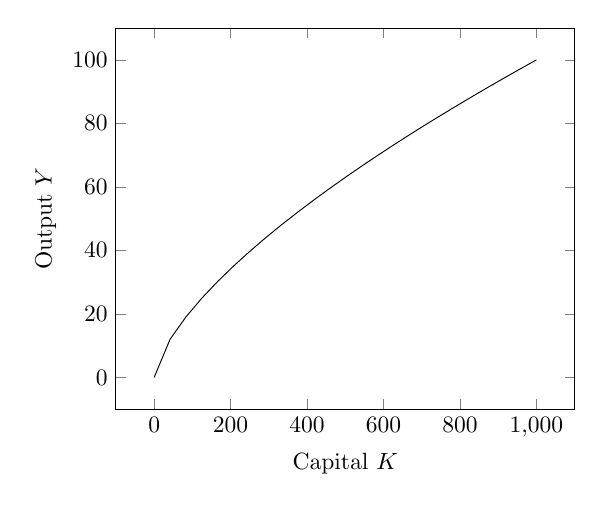
\begin{tikzpicture}[scale=0.85]
\begin{axis}[xlabel={Capital $K$},ylabel={Output $Y$}]
\addplot[domain=0:1000,black]
{(x^(2/3))};
%\addplot[domain=0:1000,black]
%{(x^(1/3))};
\end{axis}
\end{tikzpicture}
\caption{Plot of $Y$ against $K$ holding $L$ constant}
\end{subfigure}
\hspace{2ex}
\begin{subfigure}[b]{0.5\textwidth}
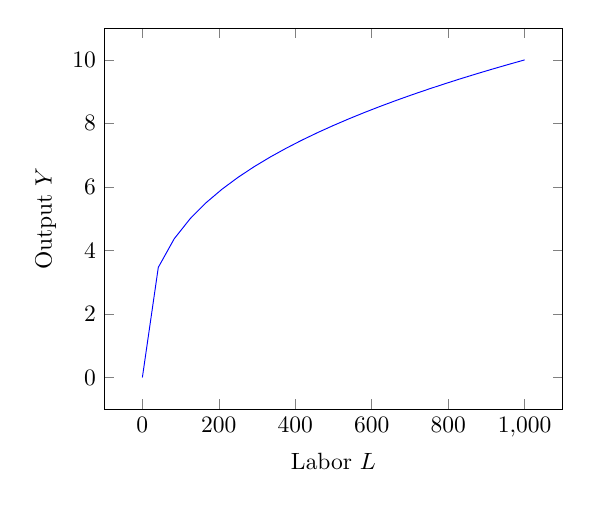
\begin{tikzpicture}[scale=0.85]
\begin{axis}[xlabel={Labor $L$},ylabel={Output $Y$}]
%\addplot[domain=0:1000,black]
%{(x^(2/3))};
\addplot[domain=0:1000,blue]
{(x^(1/3))};
\end{axis}
\end{tikzpicture}
\caption{Plot of $Y$ against $L$ holding $K$ constant}
\end{subfigure}
\caption{Y Increasing in K and L at a Declining Rate}
\end{figure}

This requires us to find the second derivatives.

\begin{align*}
\frac{\partial^2 Y} {\partial K^2} &= \bar{A} (\alpha (\alpha - 1) K^{\alpha - 2}) L^{1-\alpha} < 0\\
\frac{\partial^2 Y}{\partial L^2} &= \bar{A} K^\alpha ((1-\alpha)(-\alpha)L^{-\alpha -1}) < 0
\end{align*}

\begin{itemize}
	\item $\frac{\partial^2 Y} {\partial K^2}  < 0$ because $(\alpha - 1)$ is negative, since we stipulated that $0 < \alpha < 1$. 
	\item $\frac{\partial^2 Y}{\partial L^2} < 0$ because $(1-\alpha)$ is negative.
\end{itemize}

\subsection{Constant Returns to Scale}

Returns to scale is \textbf{different} from Diminishing Marginal Returns. Return to scale answers the question, "If I increase \emph{all} inputs by the same proportion, what will happen to output?"

In other words, we're taking our original $K$ and $L$, and multiplying them both by the same proportion $c$. Then we investigate what happens to output.

So originally, we have

\[Y_0 = \bar{A} K^\alpha L^{1-\alpha} \]

After increases in input, we have

\begin{align*}
Y_1 &= \bar{A} (cK)^\alpha (cL)^{1-\alpha} \\
&= \bar{A} (c^\alpha)(K)^\alpha (c^{1-\alpha})(L)^{1-\alpha} \\
&= c\bar{A} K^\alpha L^{1-\alpha} \\
&= cY_0
\end{align*}

We have just shown that if I increase both $K$ and $L$ by $c$, then $Y$ gets increased by the same factor.

This is what we mean by \textbf{Constant Returns to Scale}

\section{Firms' Optimal Choice}
The question we have now is, "How much labor and capital should a firm use?"

To do this, we assume that the firm \textbf{maximizes profits}. Then we find the \textbf{optimal choice of capital} and \textbf{optimal choice of labor} that maximizes profit.

\textbf{Profit is revenue minus cost}. No shit. Expressed formally, profit $\pi$ is

\begin{align*}
\pi &= Y - rK - wL \\
&= \bar{A}K^{\alpha}L^{1-\alpha} - rK - wL
\end{align*}

Now our job is to help a firm maximize its profit.

\subsection{Optimal Choice of Capital}
We want to find the optimum level of capital $K$ and labor $L$ inputs that the firm uses. We do that one at a time.

For the optimal level of capital, we simply partially differentiate the profit function with respect to $K$ and set to $0$.

\begin{align*}
\frac{\partial \pi}{\partial K} = \bar{A} \alpha K^{\alpha - 1}L^{1-\alpha} - r &= 0\\
\bar{A} \alpha K^{\alpha - 1}L^{1-\alpha} &= r
\end{align*}

Now we know that the firm must set \emph{something} to be equal to rent $r$ in order to use the optimum amount of capital. What is that \emph{something}? Let's find out.

Let's partial differentiate output $Y$ with respect to $K$.

\[ \frac{\partial Y}{\partial K} = \bar{A} \alpha K^{\alpha - 1}L^{1-\alpha} \]

Does this look familiar? Why of course it does! It's the animal on the LHS of the rent equation. Since this is the partial derivative of $Y$ with respect to $K$, this is the \textbf{Marginal Product of Capital (MPK)} -- the extra amount of output that is produced per unit of extra capital when a small amount of capital is added, \emph{holding all other inputs constant}.

Hence, in order to find the optimum level of capital, all the firm needs to do is to set \textbf{rent} equal to \textbf{Marginal Product of Capital}

\begin{align*}
\bar{A} \alpha K^{\alpha - 1}L^{1-\alpha} &= r \\
MPK &= r
\end{align*}

That makes intuitive sense -- the additional benefit from one additional unit of capital should equal the additional cost incurred. Remember \emph{marginal benefit equals marginal cost}? In this case, MPK is the marginal benefit. $r$ is the marginal cost.

\subsection{Optimal Choice of Labor}
We can do the same for labor.

\begin{align*}
\frac{\partial \pi}{\partial L} = \bar{A} \alpha K^{\alpha}(1-\alpha)L^{-\alpha} - w &= 0\\
\bar{A} \alpha K^{\alpha}(1-\alpha)L^{-\alpha} &= w\\
\end{align*}

Again, we show that the LHS of the equation is the \textbf{Marginal Product of Labor (MPL)}

\[ \frac{\partial Y}{\partial L} = \bar{A} \alpha K^{\alpha}(1-\alpha)L^{-\alpha} \]

Then in that case,

\begin{align*}
\bar{A} \alpha K^{\alpha}(1-\alpha)L^{-\alpha} &= w\\
MPL &= w
\end{align*}

Again, this makes intuitive sense. Marginal benefit of labor should equal marginal cost right?

\subsection{Curves}
The demand curve in capital market and labor markets then look like this

\begin{figure}[ht!]
\begin{subfigure}[b]{0.5\textwidth}
\begin{tikzpicture}[scale=0.85]
\begin{axis}[xlabel={Capital $K$},ylabel={Rent $r$}]
\addplot[domain=0:10,black]
{(x^(1/3-1))};
%\addplot[domain=0:1000,black]
%{(x^(1/3))};
\end{axis}
\end{tikzpicture}
\caption{Plot of $r$ against $K$ holding $L$ constant}
\end{subfigure}
\hspace{2ex}
\begin{subfigure}[b]{0.5\textwidth}
\begin{tikzpicture}[scale=0.85]
\begin{axis}[xlabel={Labor $L$},ylabel={Wages $w$}]
%\addplot[domain=0:1000,black]
%{(x^(2/3))};
\addplot[domain=0:10,blue]
{(x^(-1/3))};
\end{axis}
\end{tikzpicture}
\caption{Plot of $w$ against $L$ holding $K$ constant}
\end{subfigure}
\caption{Y Increasing in K and L at a Declining Rate}
\end{figure}

These curves are evident from the equations we derived in the two sections above. Try them!

\section{Share of Output}

To find out how much we are paying laborers, we simply \textbf{multiply wages per worker with number of workers}. Why? If you pay each worker $w$ dollars, and there are $L$ workers, then they earned $wL$ dollars in total.

The share of GDP that goes to workers is then

\begin{align*}
wL &= \bar{A}K^{\alpha}(1-\alpha)L^{-\alpha} * L\\
&= (1-\alpha)\bar{A}K^{\alpha}L^{1-\alpha} \\
&= (1-\alpha)Y
\end{align*}

So labor $L$ eats up $(1-\alpha)$ of Y. Set $\alpha = \frac{1}{3}$ and we get the $wL = \frac{2}{3}Y$ statement that \jon used.

Similarly, for capital,

\begin{align*}
rK &= \bar{A}(\alpha)K^{\alpha-1}L^{1-\alpha} * K\\
&= (\alpha)\bar{A}K^{\alpha}L^{1-\alpha} \\
&= (\alpha)Y
\end{align*}

Capital $K$ eats up $\alpha$ of Y. Set $\alpha = \frac{1}{3}$ and we see that $rK = \frac{1}{3}Y$. 

If $Y = rK + wL$, then firms are earning zero (normal) profits. Why so? Because we assumed \textbf{perfect competition}, and under perfect competition firms earn only normal profits!

\section{Output Per Capita}

In comparing different countries, we rarely compare GDP in its entirety. Instead, we're more concerned about \textbf{GDP per capita} since that gives us a better idea of how much a person in that country can consume. After all, there's not too much point in having a country with a very high GDP but an even higher population -- a single person in that country still remains poor.

To analyze this, we define \textbf{output per capita} as $y = \frac{Y}{L}$, and \textbf{capital per capita} as $k = \frac{K}{L}$

Then,

\[ y = \frac{Y}{L} = \frac{\bar{A}K^{\alpha}L^{1-\alpha}}{L} = \bar{A}K^{\alpha} \]

We find that output per capita is determined by two factors -- productivity and capital per person. This becomes a model that we can test empirically.

\end{document}